\section{Simulated Experiments}
\label{sec:exp}
\label{sec:setup}

The shaded cells in Table~\ref{tab:summary} mark the models that place
structure at the source of uncertainty. Each shaded model attains the best
value among the learned estimators shown, including ties.

\subsection{Clean events: learning to count from a terminal reward}
\label{sec:rl}
\label{sec:boundary}
We train policies with advantage actor-critic on clean sequences of length
10, using terminal reward as the training signal. Cue and monotone controls
test simpler memory tasks under the same setup.

At the common budget of $7.68$ million environment steps, four of five
phase-rotation seeds and one of five Transformer seeds reach the parity
threshold (Figure~\ref{fig:reward}a). On $\Z_3$, all five seeds of both
models reach the threshold, and phase rotation reaches both tasks'
thresholds sooner in median steps (Figure~\ref{fig:reward}b and
Table~\ref{tab:main}). After
training on lengths 4 through 14, phase rotation reaches $1.00$ on parity
and $0.90$ on $\Z_3$ at length 40.
\label{sec:lengthgen}
\begin{table}[tbp]
\centering\small
\caption{Learning from terminal reward on clean sequences of length 10.
Final success is the mean at the end of training over five seeds.
Crossing means reaching $0.90$ greedy success on parity or $0.70$ on $\Z_3$.
The median step count includes runs censored at their training budget
($7.68$M steps for GRU, LSTM, and Born, and $20.48$M for the Transformer).
The seed count uses the common budget of $7.68$M steps.}
\label{tab:main}
\begin{tabular}{llrrrr}
\toprule
Task & Measure & GRU & LSTM & Transformer & Born \\
\midrule
Cue & Final success & 1.00 & 1.00 & 1.00 & 1.00 \\
Monotone & Final success & 1.00 & 1.00 & 1.00 & 1.00 \\
\midrule
$\Z_2$ & Final success & .50 & .50 & .883 & .901 \\
      & Median crossing steps & $>$7.68M & $>$7.68M & 15.7M & 2.6M \\
      & Seeds crossing by $7.68$M & 0/5 & 0/5 & 1/5 & 4/5 \\
$\Z_3$ & Final success & .40 & .33 & .975 & .997 \\
      & Median crossing steps & $>$7.68M & $>$7.68M & 2.4M & 0.26M \\
      & Seeds crossing by $7.68$M & 0/5 & 0/5 & 5/5 & 5/5 \\
\bottomrule
\end{tabular}
\end{table}

Appendix~\ref{app:clean} gives the protocols and learning curves' summary
statistics.

\begin{figure}[!htbp]
\centering
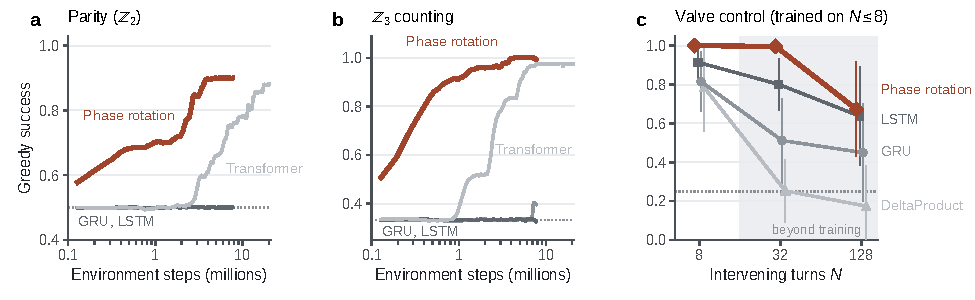
\includegraphics[width=\linewidth]{figures/fig_reward.pdf}
\caption{(a, b)~Greedy success on length-10 parity and $\Z_3$ counting is
plotted against millions of environment steps on a log scale for phase
rotation (337 and 369 parameters), the Transformer (5.9k, 20.48M-step budget),
the GRU (1.1k), and the LSTM (1.5k).
Curves show five-seed means with a five-point moving average.
(c)~Points and bars show five-seed means and sample SDs for valve success at
$N=8,32,128$ for phase rotation, the validation-selected LSTM ($H=16$) and
GRU ($H=64$), and the DeltaProduct adapter.
Dotted lines mark chance success, and shading in (c) marks horizons beyond
the training range $N\leq8$.}
\label{fig:reward}
\end{figure}

\myparagraph{The input-set angle.}
In a matched parity ablation, a diagonal complex recurrent model with a
fixed unit-modulus rotation and a squared-amplitude readout averages
$0.66$ accuracy at length 10. Setting the angle from the input raises
accuracy to $0.996$ at the same width and training budget
(Appendix~\ref{app:lru}). The input-conditioned model reaches $0.57$ at
length 20 without stabilizers. Normalization and the angle penalty target
accumulating angular error (Section~\ref{sec:stab}). Phase-advance and
readout ablations link the gains to the phase carried by the transition.
On frozen recurrent states, the squared-amplitude readout gives the
highest clean parity accuracy at length 80 (Appendix~\ref{app:clean-probes}).

\phantomsection
\myparagraph{Using the count to operate a valve.}
\label{sec:transfer}
In the four-position valve task, the policy sees the initial pointer and the
target, then receives cues for the intervening commands and their outcomes.
It makes corrective turns and selects the finish action. Training uses
1--8 intervening turns and terminal reward, and $N$ denotes the number of
intervening turns at evaluation.

The re-tuned comparison gives every family three times the original tuning
budget and a wider learning-rate grid, with a width sweep for the GRU and
LSTM. Phase rotation reaches $1.000$ success at $N=8$ and $0.997$ at $N=32$, four
times the longest training horizon, compared with $0.915$ and $0.801$ for
the best budget-matched baseline (Table~\ref{tab:valve}, Figure~\ref{fig:reward}c).
At $N=128$, sixteen times the longest training horizon, phase rotation
reaches $0.673$ and the best learned baseline reaches $0.684$. The
programmed counter succeeds at every horizon. Appendix~\ref{app:valve}
gives the tuning protocol and original-budget results.

\begin{table}[!htbp]
\centering\small
\caption{Re-tuned valve control after training on 1--8 intervening turns.
Greedy success is mean $\pm$ sample SD over five seeds, with 4,096
episodes per seed and horizon. LR is the validation-selected learning rate.}
\label{tab:valve}
\setlength{\tabcolsep}{4pt}
\begin{tabular}{@{}llrrrr@{}}
\toprule
Memory type & Policy & LR & $N=8$ & $N=32$ & $N=128$ \\
\midrule
Phase rotation & Phase rotation ($H=16$) & 0.003 & \textbf{1.000}\,$\pm$\,0.000 & \textbf{0.997}\,$\pm$\,0.005 & 0.673\,$\pm$\,0.244 \\
\midrule
\multirow{6}{*}{Gated recurrence} & LSTM ($H=16$) & 0.01 & 0.915\,$\pm$\,0.106 & 0.801\,$\pm$\,0.136 & 0.637\,$\pm$\,0.253 \\
 & LSTM ($H=32$) & 0.01 & 0.796\,$\pm$\,0.269 & 0.735\,$\pm$\,0.249 & \textbf{0.684}\,$\pm$\,0.284 \\
 & LSTM ($H=64$) & 0.003 & 0.669\,$\pm$\,0.228 & 0.633\,$\pm$\,0.183 & 0.559\,$\pm$\,0.157 \\
 & GRU ($H=16$) & 0.003 & 0.344\,$\pm$\,0.102 & 0.291\,$\pm$\,0.121 & 0.285\,$\pm$\,0.122 \\
 & GRU ($H=32$) & 0.01 & 0.737\,$\pm$\,0.205 & 0.379\,$\pm$\,0.099 & 0.296\,$\pm$\,0.101 \\
 & GRU ($H=64$) & 0.01 & 0.815\,$\pm$\,0.156 & 0.512\,$\pm$\,0.219 & 0.450\,$\pm$\,0.253 \\
\midrule
State-tracking layer & DeltaProduct adapter ($H=16$) & 0.003 & 0.784\,$\pm$\,0.228 & 0.253\,$\pm$\,0.163 & 0.174\,$\pm$\,0.208 \\
\midrule
Categorical & Learned cyclic counter ($H=16$) & 0.003 & 0.553\,$\pm$\,0.109 & 0.549\,$\pm$\,0.113 & 0.552\,$\pm$\,0.119 \\
\bottomrule
\end{tabular}
\end{table}


\subsection{One protocol, rising uncertainty}
\label{sec:sweep}
We start from an exact pointer on a four-position valve, then replace each
delivered turn token with a uniformly drawn alternative with probability $r$.
The increments regime delivers every token, while the missing regime erases
bursts and supplies noisy pointer readings.

Each learned model trains at the test misread rate on lengths $6$, $10$,
and $14$ for 3{,}000 Adam updates with batch size 96 and gradient clipping
at norm 1. Two tuning seeds evaluate the learning-rate grid
$\{10^{-3},3\times 10^{-3},10^{-2}\}$. Validation NLL selects the rate
for dense and terminal labels, and validation accuracy selects it for
terminal reward. We report final-state NLL and accuracy over five test
seeds and 1{,}024 episodes per seed and cell.

Table~\ref{tab:sweep} compares the training signals at $L=40$. On clean
inputs with a terminal label or reward, the measured-angle rotation and
the cyclic filters reach $1.000$ accuracy through $L=160$, while the GRU,
LSTM, and learned-angle rotation stay at chance.

\begin{table}[!htbp]
\centering\small
\caption{Increments regime at $L=40$. Each cell gives mean terminal
NLL (nats) / accuracy over five test seeds. Appendix~\ref{app:sweep}
reports the full sweep and NLL standard deviations.}
\label{tab:sweep}
\setlength{\tabcolsep}{3pt}
\begin{tabular}{@{}lrrrrrr@{}}
\toprule
& \multicolumn{3}{c}{$r=0$} & \multicolumn{3}{c}{$r=0.01$} \\
\cmidrule(lr){2-4}\cmidrule(l){5-7}
Estimator & Dense & Terminal & Reward & Dense & Terminal & Reward \\
\midrule
GRU & $0.000\,/\,1.000$ & $1.386\,/\,0.255$ & $7.503\,/\,0.255$ & $1.062\,/\,0.682$ & $1.387\,/\,0.251$ & $7.510\,/\,0.252$ \\
LSTM & $0.000\,/\,1.000$ & $1.386\,/\,0.255$ & $1.634\,/\,0.250$ & $1.159\,/\,0.679$ & $1.386\,/\,0.257$ & $1.937\,/\,0.242$ \\
Phase rotation (learned angle) & $0.003\,/\,1.000$ & $1.387\,/\,0.255$ & $2.418\,/\,0.244$ & $1.412\,/\,0.417$ & $1.387\,/\,0.252$ & $2.365\,/\,0.244$ \\
Phase rotation (measured angle) & $0.000\,/\,1.000$ & $0.000\,/\,1.000$ & $0.002\,/\,1.000$ & $1.309\,/\,0.683$ & $1.161\,/\,0.683$ & $2.494\,/\,0.683$ \\
Cyclic filter (token-constrained) & $0.000\,/\,1.000$ & $0.000\,/\,1.000$ & $0.000\,/\,1.000$ & $5.839\,/\,0.683$ & $5.839\,/\,0.683$ & $5.839\,/\,0.683$ \\
Cyclic filter (unconstrained) & $0.000\,/\,1.000$ & $0.000\,/\,1.000$ & $0.002\,/\,1.000$ & $0.967\,/\,0.683$ & $0.971\,/\,0.683$ & $2.379\,/\,0.683$ \\
Cyclic filter (misread-aware) & $0.012\,/\,1.000$ & $0.011\,/\,1.000$ & $0.314\,/\,1.000$ & $0.966\,/\,0.683$ & $0.966\,/\,0.683$ & $0.972\,/\,0.683$ \\
\midrule
Matched Bayes & $0.000\,/\,1.000$ & $0.000\,/\,1.000$ & $0.000\,/\,1.000$ & $0.965\,/\,0.683$ & $0.965\,/\,0.683$ & $0.965\,/\,0.683$ \\
\bottomrule
\end{tabular}
\end{table}


At $r=0.01$ and $L=40$, the token-constrained filter matches Bayes in
accuracy. Its NLL rises because it treats reported shifts as certain and
assigns near-zero probability to the true position if misreads change the
final residue. We floor probabilities at $10^{-8}$ for NLL. The misread-aware
filter reaches terminal-label NLL of $0.966$, compared with $5.839$ for
the token-constrained filter and $0.965$ for matched Bayes
(Figure~\ref{fig:sweep}a). With missing tokens and noisy readings at $r=0.3$
and $L=160$, it matches Bayes at $1.263$ NLL under state labels and leads
the learned models at $1.637$ under reward (Figure~\ref{fig:sweep}c).
Appendix~\ref{app:sweep} gives the full sweep.

\begin{figure}[!htbp]
\centering
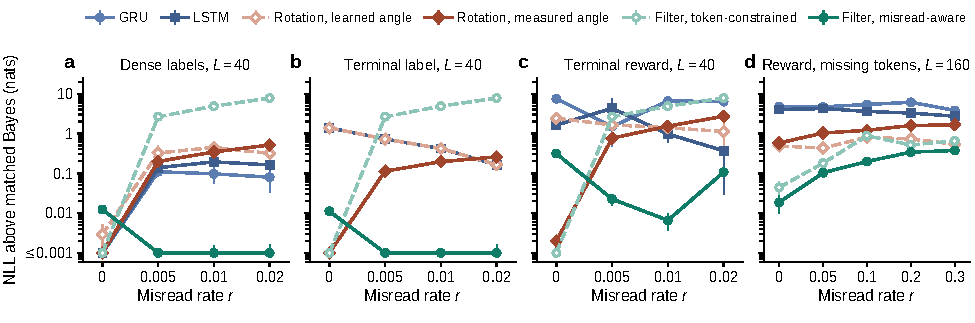
\includegraphics[width=\linewidth]{figures/fig_sweep.pdf}
\caption{Excess test NLL over matched Bayes versus token misread rate $r$.
(a, b)~The increments regime uses a terminal label and terminal reward,
respectively, at $L=40$, and (c) uses terminal reward with missing tokens
and pointer readings at $L=160$.
Points and bars show the mean and sample SD of NLL differences paired across
five test seeds, with values below $0.001$ nats at the floor of the log axis.
The thick line marks the misread-aware filter, the dashed line with open
markers marks the token-constrained filter, and grey lines show the GRU and
LSTM.}
\label{fig:sweep}
\end{figure}

\subsection{Noisy events: inferring the event before counting}
\label{sec:noisy}
We replace the observed bit with a 16-dimensional Gaussian feature vector.
The learned cyclic counter predicts event probabilities and mixes exact
shifts of the count belief. It reaches $0.994$ accuracy at $L=160$ for
$k=2,3,4$ (Table~\ref{tab:noisy}).

A learned-angle rotation represents each noisy cue by a single angle.
The cue can support multiple events, so a wrong increment shifts the
estimate and later updates accumulate these errors. With an angle penalty,
accuracy approaches chance by length 40 for $k=2,3$. At $k=4$ and $L=160$,
enforcing exact multiples of $2\pi/k$ raises accuracy from $0.248$ to
$0.562$, compared with $0.756$ for the width-32 LSTM. The cyclic counter
carries event uncertainty forward by assigning probabilities to the
possible shifts.

\begin{table}[!t]
\centering\small
\caption{Counting with noisy event features: greedy accuracy at the longest
training length ($L=14$) and at $L=160$, mean (SD) over five seeds. Chance is
$1/k$. Appendix~\ref{app:additional} reports all lengths and further baselines.}
\label{tab:noisy}
\setlength{\tabcolsep}{4pt}
\begin{tabular}{lcccccc}
\toprule
& \multicolumn{2}{c}{$k=2$} & \multicolumn{2}{c}{$k=3$} & \multicolumn{2}{c}{$k=4$} \\
\cmidrule(lr){2-3}\cmidrule(lr){4-5}\cmidrule(lr){6-7}
Model & $L=14$ & $L=160$ & $L=14$ & $L=160$ & $L=14$ & $L=160$ \\
\midrule
Cyclic counter & \textbf{.999} (.001) & \textbf{.994} (.002) & \textbf{.999} (.001) & \textbf{.994} (.002) & \textbf{.999} (.001) & \textbf{.994} (.002) \\
LSTM, width 32 & .947 (.113) & .933 (.118) & .967 (.071) & .944 (.075) & .765 (.345) & .756 (.338) \\
Born, hard angles & .492 (.021) & .499 (.015) & .841 (.283) & .699 (.214) & .884 (.079) & .562 (.081) \\
Born, soft penalty & .701 (.048) & .503 (.009) & .719 (.019) & .335 (.010) & .689 (.092) & .248 (.008) \\
\bottomrule
\end{tabular}
\end{table}


\subsection{Missing events: estimating the belief}
\label{sec:feedback}
We train estimators on four-position valve histories with a state label at
each step. Visible tokens give the exact turn, and occasional noisy pointer
readings correct the belief during histories with missing turns. The
token-constrained filter uses the known shift on visible turns, and the
unconstrained filter learns shift probabilities on every step.

On test histories with four consecutive missing turns and a pointer every
twelve steps, the token-constrained filter reaches $0.937$ NLL, compared with
$0.982$ for phase rotation and $1.011$ for the GRU. Both cyclic filters
achieve near-zero circular regret. At length 80, the token-constrained
filter's NLL falls from $1.361$ immediately before a reading to $0.591$
at the reading.

Table~\ref{tab:feedback} compares estimation and default-planner utility
on the same histories. Nominal Bayes uses the training parameters, and
matched Bayes uses the test parameters. Both compute posteriors from the
same observations as the learned estimators. The tests include shifts in
turn probabilities and pointer reliability. The token-constrained filter
comes within $0.0168$ nats of matched Bayes and gives lower NLL than
nominal Bayes ($0.937$ versus $0.944$).

\begin{table}[!htbp]
\centering\small
\caption{Cyclic filters give the lowest NLL and highest shared-planner utility
among learned estimators. The table averages five seeds, lengths 40 and 80, and the nominal,
event-rate shift, and pointer-noise shift conditions. Each history has four-step
bursts of missing turns and a pointer every twelve steps. Utility is scaled to
100 points. The last two columns give paired differences from matched Bayes
(mean $\pm$ sample SD). Circular regret is excess expected distance relative
to the best point estimate under matched Bayes.}
\label{tab:feedback}
\setlength{\tabcolsep}{2.7pt}
\begin{tabular}{llrccccrr}
\toprule
& & & \multicolumn{3}{c}{Estimation} & Control
& \multicolumn{2}{c}{Gap to matched Bayes} \\
\cmidrule(lr){4-6}\cmidrule(lr){7-7}\cmidrule(lr){8-9}
Prior & Estimator & Params & Acc.\,$\uparrow$ & NLL\,$\downarrow$
& Regret\,$\downarrow$ & Utility (pts) & $\Delta$NLL & $\Delta$Utility (pts) \\
\midrule
None & GRU & 1,844 & .634 & 1.011 & .0053 & 62.3
& $+.091\pm.006$ & $-1.05\pm0.48$ \\
Phase rotation & \shortstack[l]{Squared-amplitude\\readout} & 1,088 & .623 & .982 & .0067 & 62.3
& $+.061\pm.038$ & $-1.01\pm0.57$ \\
\midrule
\multirow{2}{*}{Cyclic filter} & Unconstrained & 196 & .634 & .938 & .0000 & 62.9
& $+.018\pm.003$ & $-0.46\pm0.32$ \\
& Token-constrained & 196 & .634 & \textbf{.937} & \textbf{.0000} & \textbf{63.0}
& $\mathbf{+.017\pm.002}$ & $\mathbf{-0.36\pm0.46}$ \\
\midrule
\multirow{2}{*}{Exact Bayes} & Nominal & 0 & .634 & .944 & .0000 & 62.7
& $+.024\pm.003$ & $-0.63\pm0.38$ \\
& Matched (ref.) & 0 & .641 & .920 & .0000 & 63.3 & --- & --- \\
\bottomrule
\end{tabular}
\end{table}


\subsection{Acting on the belief with a shared planner}
\label{sec:regimes}
The planner starts from each estimator's final belief and a target. It
chooses a turn, a pointer reading, or the finish action to maximize success
minus action costs. We vary the horizon, reading cost, and reading reliability
with the estimators fixed.

In the default setting, the token-constrained filter reaches $63.0$ utility
points, compared with $62.3$ for both the GRU and phase rotation, $62.7$
for nominal Bayes, and $63.3$ for matched Bayes (Table~\ref{tab:feedback}).
Both cyclic filters match or exceed the GRU in all
75 settings, with a positive paired bootstrap interval for the constrained
filter in 47 (Figure~\ref{fig:regimes}). Both retain at least $95\%$ of the
attainable gain in settings with at least ten points of headroom. The
differences in belief primarily affect the choice to read the pointer.
Appendix~\ref{app:regimes} gives the planner grid and sensing comparisons.

\begin{figure}[!htbp]
\centering
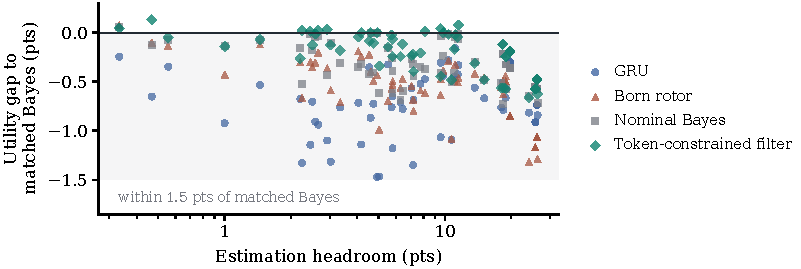
\includegraphics[width=\linewidth]{figures/fig_regimes.pdf}
\caption{Utility across 75 planner regimes, each averaged over six test
conditions and five seeds.
(a)~For the GRU, phase rotation, and the token-constrained filter in each
headroom group, the dot and bar show the median and interquartile range of
retained share across regimes.
Headroom is the utility gain of matched Bayes over a uniform belief, grouped
as below 3 points (12 regimes), 3 to under 10 points (23), and at least 10
points (40).
Dashed and dotted lines mark $100\%$ and $95\%$ retained, respectively.
(b)~The token-constrained filter's mean gain over the GRU is plotted against
headroom on a log scale with 95\% paired seed-bootstrap intervals, with filled
points for the 47 intervals above zero and open points for the 28 intervals
including zero.}
\label{fig:regimes}
\end{figure}

Cheap, reliable readings make the sensing decision sensitive to belief quality.
An overconfident belief lowers the estimated value of taking a reading. With a
two-action horizon, a $0.02$ reading cost, and reliability $0.95$, the GRU
belief leads to $0.64$ readings per episode, compared with $0.84$ for matched
Bayes. The cyclic filters preserve sensing utility across the grid. The GRU
falls below the uniform-belief baseline in three settings, by up to $0.92$
percentage points.
